\documentclass[a4j]{jarticle}
    \usepackage[dvipdfmx]{graphicx}
    \usepackage[ top=25truemm,bottom=25truemm,left=25truemm,right=25truemm]
    {geometry}
    \usepackage{ascmac}
    \usepackage{array}
    \usepackage{here}
    \usepackage{url}
    \usepackage{listings, jlisting}
    \usepackage[subrefformat=parens]{subcaption}
    \renewcommand{\lstlistingname}{リスト}
\lstset{language=c,
  basicstyle=\ttfamily\scriptsize,
  commentstyle=\textit,
  classoffset=1,
  keywordstyle=\bfseries,
  frame=tRBl,
  framesep=5pt,
  showstringspaces=false,
  numbers=left,
  stepnumber=1,
  numberstyle=\tiny,
  tabsize=4
}

\makeatletter
\def\@thesis{プログラミング演習 レポート}
\def\id#1{\def\@id{#1}}
\def\department#1{\def\@department{#1}}

\def\@maketitle{
\begin{center}
{\huge \@thesis \par} %修士論文と記載される部分
\vspace{10mm}
{\LARGE\bf \@title \par}% 論文のタイトル部分
\vspace{10mm}
{\Large \@date\par}	% 提出年月日部分
\vspace{20mm}
{\Large \@department \par}	% 所属部分
{\Large 学籍番号 \@id \par}	% 学籍番号部分
\vspace{10mm}
{\Large 氏名 \@author}% 氏名 
\end{center}
\par\vskip 1.5em
}

\title{アナログ時計}
\date{提出期限 2020年11月24日 17:00 \\ 提出日 2020年11月24日}
\department{組番号 408}
\id{17406}
\author{金澤雄大}

    \begin{document}
    \maketitle
    \thispagestyle{empty}
    \clearpage
    \addtocounter{page}{-1}
    \section{目的}
    後期のプログラミング演習で学習した内容の理解度を確認するためにアナログ時計のアプリケーションを作成する.

    \section{実行環境}
    実行環境を\ref{env}に示す.gccとは「GNU Compiler Collection」の略称で,GNUプロジェクトが公開しているコンパイラのことである.
    makeはMakefileにプログラムのコンパイルやリンクの方法を指示することで,コンパイルを簡単に行うことができるツールのことである.
    makeを用いることは,gccコンパイル時に,長いオプションを入力しなくてよい,ファイルの更新を取得して必要なものだけをコンパイルしてくれる
    という利点がある.

    \begin{table}[H]
      \caption{実行環境}
    \label{env}
    \begin{center}
        \begin{tabular}{c|l}\hline
          CPU & Intel(R) Core(TM) i7-6500U 2.50GHz  \\ 
          メモリ & 16.0GB DDR4 \\
          OS & Microsoft Windows 10 Home \\
          gcc &  version 9.3.0 \\
          make & version 4.3 \\ \hline
        \end{tabular}
    \end{center}
    \end{table}

    \section{アプリケーションの説明}
    \label{s3}
    図\ref{clock}に示すアナログ時計のアプリケーションを作成した.
    時計の表示にはライトモードとダークモードの2種類がある.ライトモードとは白を基調とした
    画面表示のことであり,ダークモードは黒を基調とした画面表示のことである.図\ref{clock}\ref{light}はライトモードのときの時計の表示例,図\ref{clock}\ref{dark}は
    ダークモードのときの時計の表示例である.モードの切り替えは,時計アプリのウィンドウをマウスで左クリックすることで行うことができる.

        \begin{figure}[H]
          \begin{minipage}{0.5\hsize}
           \begin{center}
            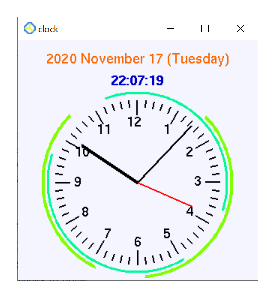
\includegraphics[scale=1.2]{light.eps}
           \end{center}
           \subcaption{ライトモードの時計}
           \label{light}
          \end{minipage}
          \begin{minipage}{0.5\hsize}
           \begin{center}
            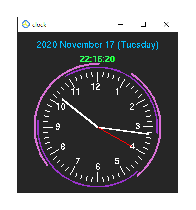
\includegraphics[scale=1.8]{dark.eps}
           \end{center}
           \subcaption{ダークモードの時計}
           \label{dark}
          \end{minipage}
          \caption{時計のアプリケーション}
          \label{clock}
         \end{figure}

          このアプリでは次に示すものを画面に描画する.アナログ時計の縁は内側と外側があり,回転している.
         回転方向は外側が時計回り,内側が反時計周りである.
         \begin{itemize}
          \item アナログ時計
          \item アナログ時計の縁
          \item 年,月,日,曜日,時,分,秒の文字列 
        \end{itemize}
          また,レポートでは伝わらないが,ライトモードとダークモードでは画面に描画している
         アナログ時計および文字列の色が異なる.表\ref{color}に2つのモードにおける色の設定を示す.

         \begin{table}[H]
          \caption{色の設定}
        \label{color}
        \begin{center}
            \begin{tabular}{c|c|c}\hline
              描画内容 & ライトモードでの色 & ダークモードでの色 \\ \hline
              背景色 & 白 & 黒 \\
              年 月 日(曜日) &  オレンジ & ライトブルー \\
              時:分:秒 & 青 & 緑 \\
              時計の針(分針,時針)およびインデックス & 黒 & 白 \\
              時計の針(秒針) & 赤 & 赤 \\
              時計の縁(内側) & スプリンググリーン & パープル \\
              時計の縁(外側) & ライムグリーン & ピンク \\ \hline
            \end{tabular}
        \end{center}
        \end{table}

    \section{プログラムの説明}
    \ref{s3}章で述べたアプリケーションを作成するためには次に示す機能を実装しなければならない.
    本章ではこれらを実装するプログラムの説明を行う.プログラムリスト全体については付録!を参照してほしい.
    \begin{itemize}
      \item ヘッダファイルの記述,オブジェクト形式マクロの宣言
      \item 初期化設定
      \item ウィンドウのリサイズへの対応
      \item タイマーを用いた時間の更新
      \item マウス入力の制御
      \item アナログ時計の針を表示する機能
      \item アナログ時計のインデックス,文字盤を表示する機能
      \item 年,月,日,曜日,時,分,秒の文字列を表示する機能
      \item 時計の縁が回転する機能 
    \end{itemize}

    \subsection{ヘッダファイルの記述,オブジェクト形式マクロの宣言}
    プログラムの実行に必要なヘッダファイルの記述,および必要なマクロを定義する.リスト\ref{include}に
    ヘッダファイルの記述,および必要なマクロを定義したコードを示す.glut.hがc言語でOpenGLを扱う
    ためのライブラリである.また,time.hは時間の取得を行うためのライブラリである.\\
     本アプリではウィンドウサイズは320$\times$320に固定する.このため,リスト\ref{include}の8行目
    および9行目ではウィンドウのサイズを定義している.\\
     リスト\ref{include}1行目から13行目行目ではグローバル変数の定義を行っている.変数dispModeは
    ライトモード,ダークモードの管理を行うための変数である.dispModeが1のときライトモード,0のとき
    ダークモードである.dispModeのデフォルト値はライトモードなっている.変数loop1,loop2はアナログ時計の縁を回転させるための変数である.
    \begin{lstlisting}[basicstyle=\ttfamily\footnotesize, frame=single,label=include,caption=定数および変数の定義]
#include<GL/glut.h>
#include<stdio.h>
#include<time.h>
#include<math.h>
#include<string.h>

// windowのサイズを定義
#define WINDOW_W 320
#define WINDOW_H 320

int dispMode =0; // 0 : LIGHTMODE 1 : DARKMODE
double loop1=0; //use for design rotation
double loop2=0; //use for design rotation
                  \end{lstlisting}

  \subsection{初期化設定}
  メイン関数では全体の初期化および設定を行う.リスト\ref{main}にメイン関数のコードを示す.
  \begin{lstlisting}[basicstyle=\ttfamily\footnotesize, frame=single,label=main,caption=main関数]
int main(int argc,char **argv){
// 初期化処理
    // 引数処理
    glutInit(&argc,argv);
    // 初期Windowサイズ設定
    glutInitWindowSize(WINDOW_W,WINDOW_H);
    // 新規Window作成
    glutCreateWindow("clock");
    // 関数登録
    glutDisplayFunc(Display);
    glutReshapeFunc(Reshape);
    glutMouseFunc(Mouse);
    glutTimerFunc(500,Timer,0);
    // display初期化
    glutInitDisplayMode(GLUT_RGBA);
    glClearColor(0.96,0.96,1.0,1.0);
    // メインループ
    glutMainLoop();
    return 0;
}
  \end{lstlisting}   
  メイン関数の処理の説明を次に示す.
  \begin{enumerate}
    \item 引数の処理をglutInit関数で行う.本アプリでは引数は使用しないから,ここではglutInit関数に形式的に引数を渡している
    だけである(リスト\ref{main}の4行目).
    \item 最初に開くウィンドウのサイズを指定する.ウィンドウのサイズの初期設定はglutInitWindowSize関数で行う.glutInitWindowSize関数の
    引数は(横幅,縦幅)である.ここでは,オブジェクト形式マクロで定義したWINDOW\_Wを横幅,WINDOW\_Hを縦幅とする(リスト\ref{main}の6行目).
    \item 開くウィンドウのサイズが決まったから,ウィンドウを生成する.ウィンドウの生成はglutCreateWindow関数で行う.glutCreateWindow関数の引数
    として渡している文字列は図\ref{clock}において,ウィンドウの左上に表示されている文字列である.リスト\ref{main}の8行目では「clock」という文字列
    をglutCreateWindow関数に渡しているから図\ref{clock}のウィンドウの左上には「clock」と表示されている.
    \item リスト\ref{main}の10行目から13行目はイベントによって呼び出される関数を定義している.本アプリにおいて,イベント(例としてユーザーからの入力やタイマーによる時間経過)
    はループを用いて逐一見張っている仕組みではない.本アプリのイベントに対する仕組みは,普段は何もせず,イベントが起こったときにそれに応じた処理を行うものである.
    このような仕組みをイベント駆動型プログラミングという.また,呼び出される関数をコールバック関数という.リスト\ref{main}では4つイベントに対してコールバック関数を設定している.
    それぞれのコールバックの呼び出されるイベントと処理内容の概要を次に示す.
    \begin{itemize}
      \item glutDisplayFunc $\dots$ ウィンドウの表示内容を更新するDisplay関数を呼び出す.
      \item glutReshapeFunc $\dots$ ウィンドウのサイズが変更されたときに,座標系およびウィンドウのサイズに関する設定するReshape関数を呼び出す.
      \item glutMouseFunc $\dots$ マウスの移動やクリックが発生したときに,マウスの移動やクリックに対する処理を行うMouse関数を呼び出す.
      \item glutTimerFunc $\dots$ 第一引数の時間(ミリ秒)が経過したときに,タイマーの処理を行うTimer関数を呼び出す.
    \end{itemize}
    \item リスト\ref{main}の15行目から16行目では生成したウィンドウに初期の背景を描画する処理を行っている.glutInitDisplayMode関数は色の指定を
    どのように行うかを設定している.ここでは色をRGBA,つまり赤(Red),緑(Green),青(Blue),透明度(Alpha)の4つの変数で指定する設定を行っている.そして
    glClearColor関数で初期の背景を描画する処理を行っている.注意として,glClearColor関数の引数は0から1までの値で色を指定する.ここでは,すべての値が
    ほぼ1であるため,白に近い色が描画される.
    \item 初期設定が終了したから,メインのループに入る関数であるglutMainLoop関数を実行する.
  \end{enumerate}

  \subsection{ウィンドウのリサイズへの対応}
  ウィンドウのリサイズへの対応について,仕様とプログラムでの実装部分を説明する.本アプリではウィンドウのリサイズを行っても,
  元のサイズ(320$\times$320)に戻される仕様になっている.これには2つの理由がある.1つ目は,アナログ時計を描画する部分において,
  ウィンドウのサイズに応じてアナログ時計の大きさを変化させるときに,中心からの距離の指定が複雑になることを防ぐためである.
  2つ目は,文字列を表示している関数は自由に拡大縮小ができないため,画面の大きさに対して不格好な描画になってしまうためである.\\
   ウィンドウのサイズ変更イベントの処理を行う関数はReshape関数であった.リスト\ref{reshape}にReshape関数のコードを示す.
  リスト\ref{reshape}において,Reshape関数の引数は新しいウィンドウの幅,高さhである.
  \begin{lstlisting}[basicstyle=\ttfamily\footnotesize, frame=single,label=reshape,caption=Reshape関数]
void Reshape(int w,int h){
    //printf("ウィンドウの幅と高さ=%d x %d\n",w,h);
    glViewport(0,0,w,h);
    glMatrixMode(GL_MODELVIEW);
    glLoadIdentity();
    gluOrtho2D(0,w,0,h);
    glScaled(1,-1,1);
    glTranslated(0,-h,0);

    //windowサイズ固定 
    glutReshapeWindow(WINDOW_W,WINDOW_H);
}    
      \end{lstlisting} 
       Reshape関数の処理内容について説明する.ウィンドウの座標系はウィンドウを更新するたびに初期設定に戻ってしまう.ウィンドウの初期設定における
        座標系を図\ref{initzahyou}に示す.図\ref{initzahyou}の座標系では描画する図形の頂点の値を実数で与えないといけない
        ため,扱いにくい.そこで図\ref{generalzahyou}に示す座標系に設定しなおす.リスト\ref{reshape}の2行目から8行目では,
        図\ref{initzahyou}の座標系を,リスト\ref{generalzahyou}の座標系にする設定を行っている.\\
         ウィンドウサイズの固定はリスト\ref{reshape}の11行目で行っている.glutReshapeWindow関数にウィンドウの
        幅,高さを引数として渡すことで内部でウィンドウのリサイズを行うことができる.

        \begin{figure}[H]
          \begin{minipage}{0.5\hsize}
           \begin{center}
            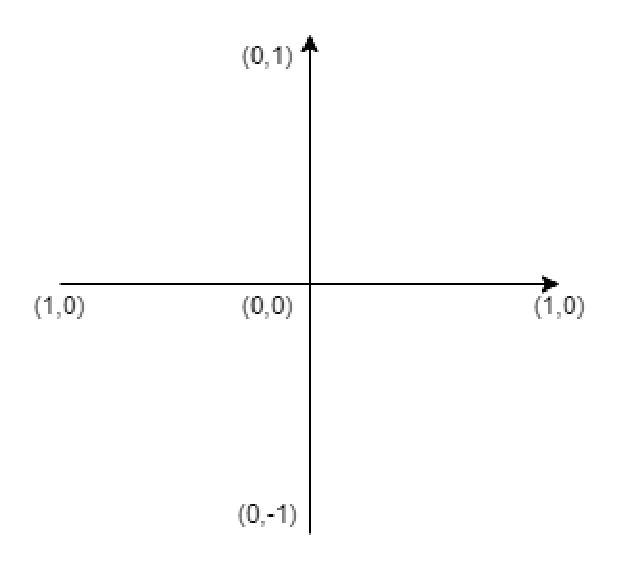
\includegraphics[scale=0.6]{czahyou.eps}
           \end{center}
           \subcaption{初期設定の座標系}
           \label{initzahyou}
          \end{minipage}
          \begin{minipage}{0.5\hsize}
           \begin{center}
            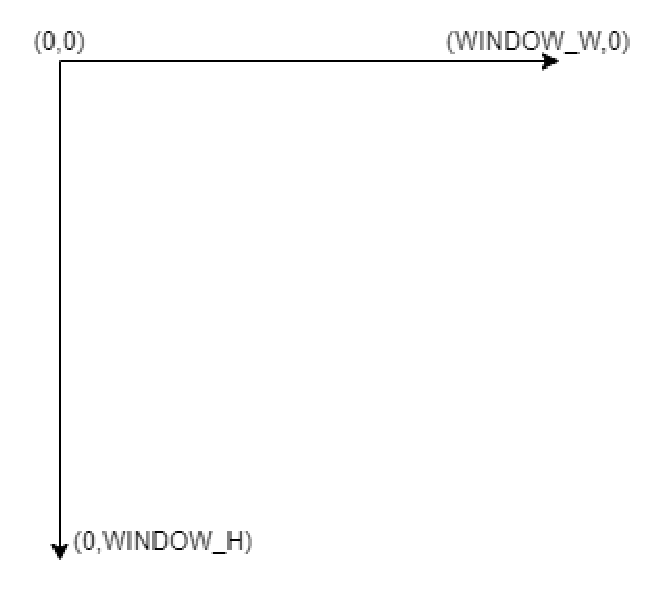
\includegraphics[scale=0.6]{zahyou.eps}
           \end{center}
           \subcaption{変換後の座標系}
           \label{generalzahyou}
          \end{minipage}
          \caption{座標系の設定}
          \label{zahyou}
         \end{figure}

    \subsection{タイマーを用いた画面描画の更新}
    タイマーによって一定時間おきに画面描画を更新する仕組みについて説明する.実装したいことは
    タイマーによって一定おきにイベントが発生することと,画面描画を更新することに切り分けられる.
    本節では,前者のタイマーによって一定おきにイベントが発生する仕組みについて説明する.後者は
    ここでは,画面描画を更新するDisplay関数がうまくやってくれると考える.\\
     第一引数の時間(ミリ秒)が経過したときに,タイマーの処理を行う関数はTimer関数であった.Timer関数の
    コードをリスト\ref{timer}に示す.Timer関数はメイン関数(リスト\ref{main})の13行目に呼ばれる.
    ここでは500ミリ秒経過後にリスト\ref{timer}のTimer関数が呼ばれる設定になっている.\\
     Timer関数の処理内容は,まず2行目でディスプレイの表示内容を更新するためのイベントを発生させるglutPostRedisplay
    関数が実行される.これによってdisplay関数が呼び出されて画面表示が更新される.次に,glutTimerFuncを
    再度実行する(リスト\ref{timer}の3行目).glutTimerFunc関数に登録されたタイマーは1度しか実行されないため,反復的に
    タイマーを利用するためにはイベントの設定を再度行う必要がある.
    
    \begin{lstlisting}[basicstyle=\ttfamily\footnotesize, frame=single,label=timer,caption=Timer関数]
void Timer(int value){
    glutPostRedisplay();
    glutTimerFunc(500,Timer,0);
}
            \end{lstlisting} 

    \subsection{マウス入力の制御}
    マウスの左クリックによってライトモードとダークモードが切り替わる仕組みについて説明する.
    マウスの移動やクリックが発生したときに,その動作に対する処理を行う関数はMouse関数であった.
    Mouse関数のコードをリスト\ref{mouse}に示す.Mouse関数の引数は,クリックされたボタンを示すb,
    ボタンの状態(押されたのか,離されたのか)を示すs,ボタンの座標(x,y)の4つである.
    \begin{lstlisting}[basicstyle=\ttfamily\footnotesize, frame=single,label=mouse,caption=Mouse関数]
void Mouse(int b,int s,int x,int y){
    if(b==GLUT_LEFT_BUTTON){
        if(s==GLUT_UP){
            if(dispMode==1){
                dispMode=0;
            }else{
                dispMode=1;
            }
        }
        if(dispMode){
            glClearColor(0.15,0.15,0.15,1.0);
        }else{
            glClearColor(0.96,0.96,1.0,1.0);
        }
    }
}
            \end{lstlisting}
       Mouse関数の処理内容について説明する.リスト\ref{mouse}の2行目から9行目では左クリックがされたときに
      dispModeを切り替える処理を行っている.リスト\ref{mouse}の2行目のif文で,イベントが起きたボタンが「左ボタン」であること
      を判定し,3行目のif文でボタンが「離された」ことを判定している.このように,マウスイベントの判定は,「左ボタンがクリックされたか」
      という事象を,イベントがあったボタンの種類,押されたのか離されたのか,という2つに分解して判定している.
      そして,5行目から8行目で2つのモードの切り替えを行っている.\\
       リスト\ref{mouse}の10行目から14行目ではdispModeの変更に伴って,背景色を変更したいから,glClearColor関数を実行する処理を行っている.

    \subsection{アナログ時計の針を表示する機能}
    画面表示を行う関数としてDisplay関数を作成し,次の機能を実装する.Display関数の設計として,画面に表示する順番がある.
    アナログ時計の描画において,最も最前面に描画するべき情報は時計の針である.次に,時計のインデックス,文字盤,
    年月日に関する文字列の3つが同程度に重要である.時計の縁はデザイン性を高めるためのものであるから最も重要度が低い.
    したがって,フロー処理においてこれらを描画する順番は箇条書きの順番と一致する.Display関数における4つの機能の実装
    プログラムの説明は,プログラムの必要な部分を抜粋して行う.このため描画する順番がわかりずらい.プログラムソース全体
    は付録!に載っているから,描画の順番は付録!の!を参照してほしい.
    \begin{enumerate}
      \item 時計の縁が回転する機能 
      \item 年,月,日,曜日,時,分,秒の文字列を表示する機能
      \item アナログ時計のインデックス,文字盤を表示する機能
      \item 時計の針を描画する機能 
    \end{enumerate}

     アナログ時計の針を表示する機能について解説する.アナログ時計の「針を表示する機能」を実装するコードを抜粋したものを
    リスト\ref{display1}に示す.リスト\ref{display1}にはDisplay関数,calPosition関数,drawLine関数の3つの関数がある.
    \begin{lstlisting}[basicstyle=\ttfamily\footnotesize, frame=single,label=display1,caption=針の描画の実装]
void Display(void){
    int i; //ループ用
    char *timestr; // 時間情報表示用文字列    
    // 画面サイズ取得
    int xc = glutGet(GLUT_WINDOW_WIDTH)/2;
    int yc = glutGet(GLUT_WINDOW_HEIGHT)/2+30; // y軸方向の中心は30ずらす.

    // 針の角度
    double thetas,thetam,thetah;
    // 針の座標
    int xs,ys,xm,ym,xh,yh;
    // 針の長さ
    int ls=80;
    int lm = 105;
    int lh = 90; 

    // 描画クリア
    glClear(GL_COLOR_BUFFER_BIT);
    
// 時間取得
    time_t tt;
    struct tm *ts;
    time(&tt);
    ts = localtime(&tt);

// 針の角度,座標を計算
    thetas = 2*M_PI*ts->tm_sec/60;
    thetam = 2*M_PI*(60*ts->tm_min+ts->tm_sec)/3600;
    thetah = 2*M_PI*(3600*(ts->tm_hour%12)+60*ts->tm_min+ts->tm_sec)/43200;
    calPosition(&xs,&ys,xc,yc,ls,thetas);
    calPosition(&xm,&ym,xc,yc,lm,thetam);
    calPosition(&xh,&yh,xc,yc,lh,thetah);

// 針を描画
    //時針描画
    if(dispMode){
    glColor3ub(255,255,255);
    }else{
    glColor3ub(0,0,0);
    }
    glLineWidth(5.0);
    drawLine(xc,yc,xh,yh);
    //分針描画
    glLineWidth(3.0);
    drawLine(xc,yc,xm,ym);
    //秒針描画
    glLineWidth(2.0);
    glColor3ub(255,0,0);
    drawLine(xc,yc,xs,ys);

    glFlush();
}

// 極座標と直交座標を変換
//極座標(r,theta)を(xc,yc)を原点とした直交座標(x,y)に変換
void calPosition(int *x,int *y,int xc,int yc,int r,double theta){
    *x = xc+r*sin(theta);
    *y = yc-r*cos(theta);
}

// lineを描画
//(x1,y1)と(x2,y2)を結ぶ直線を描画
void drawLine(int x1,int y1,int x2,int y2){
    glBegin(GL_LINES);
    glVertex2i(x1,y1);
    glVertex2i(x2,y2);
    glEnd();
};
            \end{lstlisting}
    
            Display関数の処理の内容を説明する.     
            リスト\ref{display1}の5行目および6行目では,ウィンドウの中央の座標を取得して変数xc,xyに代入している.
              glutGet関数はウィンドウや画面の情報を取得するための関数で,引数として「GLUT\_WINDOW\_WIDTH」を与えるとウィンドウの
              幅の情報が戻り値として得られる.同様に引数として「GLUT\_WINDOW\_HEIGHT」を与えることで,ウィンドウの高さの情報
              が取得できる.そして取得した値を2で割ることで,画面の中央の座標を得ることができる.6行目でycの値に30を足しているのは,
              画面中央を基準に時計を描画すると,文字列を表示する場所が狭くなってしまうためである.ycに30を足すことで,
              時計の中心をy軸方向30pixel下に移動している.\\
               リスト\ref{display1}の9行目から15行目では秒針,分針,時針の3つの描画位置を計算するための変数を定義している.\\
               リスト\ref{display1}の18行目では,画面表示をクリアな状態にするglClear関数を実行している.引数として
              与えている「GL\_COLOR\_BUFFER\_BIT」はカラーバッファとよばれる色情報を格納するメモリのことで,これを
              塗りつぶすことで,画面表示をクリアしている.\\
               時計を作成するために,時間の取得を行う.時間の取得を行っている部分はリスト\ref{display1}の21行目から
              24行目である.「time.h」の関数を用いるため,リスト\ref{include}の3行目で「time.h」を
              読み込んでいる.時間の取得はtime\_t型の変数をtime関数にわたすことで取得することができる.\\
               我々がほしい情報は現在時刻はtm構造体が保持しているため,time\_t型から変換を行う必要がある.この変換
              を行っているのが,リスト\ref{display1}の24行目である.tm構造体の構造はリスト\ref{tm}のようになっている.
              現在時間の情報の取得方法の例として,日付の情報がほしい場合は「ts-$>$tm\_mday」と記述することで取得できる.
              他の情報の取得方法もリスト\ref{tm}を参考に取得できる.

    \begin{lstlisting}[basicstyle=\ttfamily\footnotesize, frame=single,label=tm,caption=tm構造体]
struct tm{
  int tm_sec; // 秒(0~60). 60は閏秒対応のため
  int tm_min; // 分(0~59).
  int tm_hour; // 時間(0~23).
  int tm_mday; // 日(1~31).
  int tm_mon; // 1月からの通算月数(0~11).
  int tm_year; // 1900年からの通算年数.
  int tm_wday; // 曜日(0~6).0が日曜日で6が土曜日.
  int tm_yday; // 1月1日からの通算日数(0~365).
  int tm_isdst; // 夏時間が有効かどうかのフラグ.
}
            \end{lstlisting}

             時間の取得ができたから,アナログ時計の針の角度および座標を計算する.リスト\ref{display1}では27行目から32行目である.
            27行目から29行目ではそれぞれの針の角度を計算している.角度は図\ref{tokei}に示すように時計の12時の位置を0度としている.
    \begin{figure}[H]
      \centering
      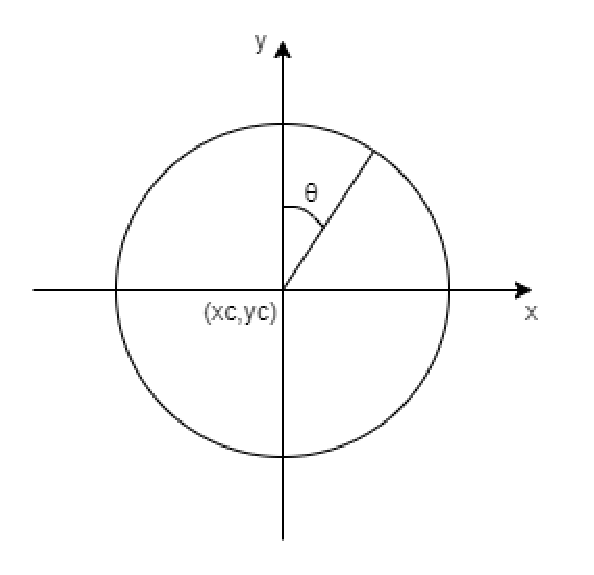
\includegraphics[scale=0.6]{tokei.eps}
      \caption{時計の針の角度}
       \label{tokei}
      \end{figure}

       時刻h時m分s秒のときの秒針の角度$\theta_s$は式(\ref{thetas})で与えられる.同様に分針の角度$\theta_m$は式(\ref{thetam}),
      分針の角度$\theta_h$は式(\ref{thetah})で計算できる.
          \begin{eqnarray}
            \label{thetas}
      \theta_s &=& \frac{2\pi s}{60}  \\
            \label{thetam}
      \theta_m &=& \frac{2\pi(60m+s)}{3600}  \\
            \label{thetah}
      \theta_h &=& \frac{2\pi(2600h+60m+s)}{43200}
        \end{eqnarray}

        角度が計算できたから,中心からの距離と角度の情報をもとに,針先の座標を計算する.針先の座標の計算はリスト\ref{display1}の
        30行目から32行目に示すようにcalPosition関数で行っている.calPosition関数の定義はリスト\ref{display1}の56行目から59行目
        にある.calPosition関数は,針先の座標を格納する変数x,yのポインタ,中心座標(xc,yc),中心からの距離r,角度thetaの6つを引数とし
        ている.計算結果は戻り値ではなくx,yに代入される.極座標($r$,$\theta$)から直交座標($x$,$y$)の変換は式(\ref{posix})および
        式(\ref{posiy})でできる.

        \begin{eqnarray}
          \label{posix}
    x &=& x_c + l \sin \theta  \\
          \label{posiy}
    y &=& y_c - l \cos \theta
      \end{eqnarray}
        
      針の座標が計算できたから,描画を行う.プログラムではリスト\ref{display1}の36行目から49行目である.36行目から40行目では,
      針の色の設定を行っている.まず,表示モードで色の場合分けがあるため,if文でdispModeでどちらのモードかを判定し,処理を分岐させる.\\
       そして,glColor3ub関数で色の設定で行う.glColor3ub関数は引数として(R,G,B)の情報を0から255の整数で与えることで色の設定が行われる.
      設定は再度glColor3ub関数で違う色に設定するまで有効である.ダークモード(dispMode=1)のとき,針の色を(255,255,255),つまり白に設定している.
      ライトモード(dispMode=0)のときは,針の色を(0,0,0),つまり黒に設定している.このため,図\ref{clock}に示したように,時針と分針が
      ライトモードのときは黒,ダークモードのときは白で表示される.秒針が赤で描画されているのは,48行目でglColor3ub関数を呼び出して,
      色を(255,0,0),つまり赤に設定してから秒針を描画しているからである.\\
       色の設定ができたから,線の太さの設定を行う.プログラムでは41,44,47行目である.41行目では,時針の太さをglLineWidth関数で設定している.
      glLineWidth関数は引数に太さを数値で与えると,値に応じた太さで線が描画させる.同様に,44行目で分針,47行目で秒針の太さを設定している.
      図\ref{clock}を見ると,それぞれの針で太さが変わっていることがわかる.\\
       時針の描画は42行目,分針の描画は44行目,秒針の描画は49行目で行っている.針の描画を行う関数はdrawLine関数である.drawLine関数は
      リスト\ref{clock}の63行目から68行目で定義している.drawLine関数は引数として2点の座標(x1,y1),(x2,y2)を与えると,この2点を
      結ぶ線を描画する機能をもつ.線を結ぶ方法は64行目のglBegin関数で画面描画を行うことを宣言する.67行目のglEnd関数はglBegin関数と
      対になる関数である.直線を描くための点はglVertex2i関数で指定する.65および66行目のように,glVertex2i関数に座標をわたすことで
      直線を描くための点を指定できる.そして,glBegin関数に「GL\_LINES」を引数として指定することで直線を描くことができる.\\
       ここまでで描画した内容はキューにためられているだけで,まだ描画されていない.このキューの内容を実行して画面に反映させる関数が
      リスト\ref{clock}の51行目のglFlush関数である.

    \subsection{アナログ時計のインデックス,文字盤を表示する機能}
    アナログ時計のインデックスおよび文字盤を表示する機能の実装について説明する.

    \begin{lstlisting}[basicstyle=\ttfamily\footnotesize, frame=single,label=indexstr,caption=インデックスと文字盤の実装]
void Display(void){
  // インデックス描画用
  double l,theta; 
  int x1,x2,y1,y2;
  char s[3];

  // ---中略---

  // インデックス描画
  for(i=1;i<=60;i++){
      if(dispMode){
        glColor3ub(255,255,255);
      }else{
        glColor3ub(0,0,0);
      }
      glLineWidth(2.0);
      l=100; // インデックスの先端を長さ110にする
      if(i%5==0){  // 5の倍数の針は長くする
      l = 90; // インデックスの終端を長さ90にする
      }
      theta = 2*M_PI*i/60;
      calPosition(&x1,&y1,xc,yc,l,theta);
      l = 110;
      calPosition(&x2,&y2,xc,yc,l,theta);
      drawLine(x1,y1,x2,y2);


      if(dispMode){
        glColor3ub(255,255,255);
      }else{
        glColor3ub(0,0,0);
      }
      if(i%5==0){ // 5の倍数のとき文字を表示
          sprintf(s,"%d",i/5);
          l =80; // 文字表示位置を80にする
          calPosition(&x2,&y2,xc,yc,l,theta);
          if(i/5<10){ // 一桁表示用
              glRasterPos2i(x2-5,y2+5);
              glutBitmapCharacter(GLUT_BITMAP_HELVETICA_18,s[0]);

          }else{ // 二桁表示用
              glRasterPos2i(x2-14,y2+5);
              glutBitmapCharacter(GLUT_BITMAP_HELVETICA_18,s[0]);
              glutBitmapCharacter(GLUT_BITMAP_HELVETICA_18,s[1]);
          }
      }
  }
}


    \end{lstlisting}

    \section{ビルド方法の説明}
    \section{実行結果とその説明}

    !付録
        \begin{thebibliography}{9}
          \bibitem{NNCT}  国立高専機構長野高専,\url{http://www.nagano-nct.ac.jp/} ,閲覧日2020年8月5日
          \end{thebibliography}
\end{document}

